\documentclass{article}
\usepackage{amsmath}
\usepackage{amssymb}
\newcommand*{\qed}{\hfill\ensuremath{\blacksquare}}
\usepackage{graphicx}
\graphicspath{{.}}

\title{Computational Linear Algebra, Module 5}
\author{Maya Shende}
\date{Due: March 21st, 2017}

\begin{document}
\maketitle

\begin{enumerate}
	\item The matrix $
	\begin{bmatrix}
		1	&0	&0\\
		0	&0	&1\\
		0	&1	&0
	\end{bmatrix}
	$ will swap rows 2 and 3, and works like this: $
	\begin{bmatrix}
		1	&0	&0\\
		0	&0	&1\\
		0	&1	&0
	\end{bmatrix}
	\begin{bmatrix}
		1	&2	&3\\
		4	&5	&6\\
		7	&8	&9
	\end{bmatrix}
	= 
	\begin{bmatrix}
		1	&2	&3\\
		7	&8	&9\\
		4	&5	&6
	\end{bmatrix}	
	$. \\
	The matrix $
	\begin{bmatrix}
		1	&0	&0\\
		0	&0	&1\\
		0	&1	&0
	\end{bmatrix}
	$ will swap rows 3 and 2, and works the same as the previous example (because the swap matrix is the same). 
	When you multiple the matrix that does the 2-3 swap with the matrix that does the 3-2 swap, you get the identity matrix back. The matrix that swaps rows $i$ and $j$ in an $n \times n$ matrix is formed by turning the identity matrix $
	\begin{bmatrix}
		\dots		&v_1		&\dots\\
		\dots 	&v_2		&\dots\\
		\vdots	&\vdots	&\vdots\\
		\dots		&v_i		&\dots\\
		\vdots	&\vdots	&\vdots\\
		\dots		&v_j		&\dots\\
		\vdots	&\vdots	&\vdots\\
		\dots		&v_n		&\dots
	\end{bmatrix}
	$ into $
	\begin{bmatrix}
		\dots		&v_1		&\dots\\
		\dots 	&v_2		&\dots\\
		\vdots	&\vdots	&\vdots\\
		\dots		&v_j		&\dots\\
		\vdots	&\vdots	&\vdots\\
		\dots		&v_i		&\dots\\
		\vdots	&\vdots	&\vdots\\
		\dots		&v_n		&\dots
	\end{bmatrix}
	$ (just swap the $i^{th}$ and $j^{th}$ rows of the identity matrix. Again, if you multiply this matrix with itself, you get the original identity matrix back.
	
	\item $
	\begin{bmatrix}
		1	&0	&0\\
		0	&1	&0\\
		0	&0	&\frac{1}{2}
	\end{bmatrix}
	$. For example, $
	\begin{bmatrix}
		1	&0	&0\\
		0	&1	&0\\
		0	&0	&\frac{1}{2}
	\end{bmatrix}
	\begin{bmatrix}
		1	&2	&3\\
		7	&8	&9\\
		4	&5	&6
	\end{bmatrix}	
	=
	\begin{bmatrix}
		1	&2	&3\\
		7	&8	&9\\
		2	&\frac{5}{2}	&3
	\end{bmatrix}	
	$. To form the $n \times n$ matrix that divides row $i$ by a value $\beta$, you just replace the 1 in the $i^{th}$ row of the identity matrix by the value $\frac{1}{\beta}$. 
	
	\item $r_A(2) = (4, 5, 6)$ and $r_A(3) = (7, 8, 9)$. 
	\item $r_A(1) \leftarrow r_A(1) - 3r_A(2)$\\
	$
	\begin{bmatrix}
		1	&-3\\
		0	&1
	\end{bmatrix}
	\begin{bmatrix}
		1	&3\\
		0	&1
	\end{bmatrix}
	= 
	\begin{bmatrix}
		1	&0\\
		0	&1
	\end{bmatrix}
	$
	\item The matrix that achieves this transformation is the identity matrix, where the $ij^{th}$ entry is $\alpha$. To make the inverse of this matrix, simply negate the $\alpha$. 
	
	\item $
	\begin{bmatrix}
		1	&0	&\dots	&0\\
		0	&1	&\dots	&0\\
		\vdots	&\vdots	&\ddots	&\vdots\\
		0	&0	&\dots	&1
	\end{bmatrix}
	\begin{bmatrix}
		a_{11}	&a_{12}	&\dots	&a_{1n}\\
		a_{21}	&a_{22}	&\dots	&a_{2n}\\
		\vdots	&\vdots	&\ddots	&\vdots\\
		a_{n1}	&a_{n2}	&\dots	&a_{nn}	
	\end{bmatrix}
	= \begin{bmatrix}
		a_{11}	&a_{12}	&\dots	&a_{1n}\\
		a_{21}	&a_{22}	&\dots	&a_{2n}\\
		\vdots	&\vdots	&\ddots	&\vdots\\
		a_{n1}	&a_{n2}	&\dots	&a_{nn}			
	\end{bmatrix}
	$. So, it is the multiplicative identity. Geometrically, if we think of our space as an n-dimensional space, we are basically multiplying n-vectors by the unit vector basis that makes up the space, so we are not changing the n original vectors at all. 
	
	\item This is because if we have $xy = 1$, then we can solve for $y$, the multiplicative inverse, by dividing by $x$, $y = \frac{1}{x} = x^{-1}$. 
	
	\item $\begin{bmatrix}
		-0.2	&0.3\\
		04	&-0.1
	\end{bmatrix}
	\begin{bmatrix}
		1	&3\\
		4	&2
	\end{bmatrix}
	= 
	\begin{bmatrix}
		-0.2+0.3(4)	&-0.2(3)+0.3(2)\\
		0.4-0.1(4)		&0.4(3)-0.1(2)
	\end{bmatrix}
	=
	\begin{bmatrix}
		1	&0\\
		0	&1
	\end{bmatrix}
	$. 
	
	\item $
	\begin{bmatrix}
		1	&3\\
		4	&2
	\end{bmatrix}
	\begin{bmatrix}
		x_1\\
		x_2
	\end{bmatrix}
	= 
	\begin{bmatrix}
		7.5\\
		10
	\end{bmatrix}	
	$
	
	\item This is true because we have applied linear operations to both sides of the constraint equations. 
	
	\item $
	\begin{bmatrix}
		4	&12\\
		4	&2
	\end{bmatrix}
	\begin{bmatrix}
		x_1\\
		x_2
	\end{bmatrix}
	= 
	\begin{bmatrix}
		30\\
		10
	\end{bmatrix}
	$
	
	\item $
	\begin{bmatrix}
		4	&12\\
		0	&10
	\end{bmatrix}
	\begin{bmatrix}
		x_1\\
		x_2
	\end{bmatrix}
	= 
	\begin{bmatrix}
		30\\
		20
	\end{bmatrix}
	$
	
	\item $
	\begin{bmatrix}
		1	&3\\
		0	&1
	\end{bmatrix}
	\begin{bmatrix}
		x_1\\
		x_2
	\end{bmatrix}
	= 
	\begin{bmatrix}
		7.5\\
		2
	\end{bmatrix}
	$
	
	\item $
	\begin{bmatrix}
		1	&0\\
		0	&1
	\end{bmatrix}
	\begin{bmatrix}
		x_1\\
		x_2
	\end{bmatrix}
	= 
	\begin{bmatrix}
		1.5\\
		2
	\end{bmatrix}
	$
	
	\item $A: 
	\begin{bmatrix}
		2	&-3	&2\\
		-2	&1	&0\\
		1	&1	&-1
	\end{bmatrix}
	\begin{bmatrix}
		x_1\\
		x_2\\
		x_3
	\end{bmatrix}
	= 
	\begin{bmatrix}
		5\\
		-1\\
		0
	\end{bmatrix}
	$. \\
	Divide $r_1$ by 2: $
	\begin{bmatrix}
		1	&\frac{-3}{2}	&1\\
		-2	&1	&0\\
		1	&1	&-1
	\end{bmatrix}
	\begin{bmatrix}
		x_1\\
		x_2\\
		x_3
	\end{bmatrix}
	= 
	\begin{bmatrix}
		\frac{5}{2}\\
		-1\\
		0
	\end{bmatrix}
	$\\
	$r_2 \leftarrow r_2 + 2r_1:
	\begin{bmatrix}
		1	&\frac{-3}{2}	&1\\
		0	&-2	&2\\
		1	&1	&-1
	\end{bmatrix}
	\begin{bmatrix}
		x_1\\
		x_2\\
		x_3
	\end{bmatrix}
	= 
	\begin{bmatrix}
		\frac{5}{2}\\
		4\\
		0
	\end{bmatrix}
	$\\
	$r_3 \leftarrow r_3 - r_1:
	\begin{bmatrix}
		1	&\frac{-3}{2}	&1\\
		0	&-2	&2\\
		0	&\frac{5}{2}	&-2
	\end{bmatrix}
	\begin{bmatrix}
		x_1\\
		x_2\\
		x_3
	\end{bmatrix}
	= 
	\begin{bmatrix}
		\frac{5}{2}\\
		4\\
		\frac{-5}{2}
	\end{bmatrix}
	$
	
	\item $r_2 \leftarrow \frac{-1}{2}r_2:
	\begin{bmatrix}
		1	&\frac{-3}{2}	&1\\
		0	&1	&-1\\
		0	&\frac{5}{2}	&-2
	\end{bmatrix}
	\begin{bmatrix}
		x_1\\
		x_2\\
		x_3
	\end{bmatrix}
	= 
	\begin{bmatrix}
		\frac{5}{2}\\
		-2\\
		\frac{-5}{2}
	\end{bmatrix}
	$. \\
	$r_3 \leftarrow r_3-\frac{5}{2}r_2:
	\begin{bmatrix}
		1	&\frac{-3}{2}	&1\\
		0	&1	&-1\\
		0	&0	&\frac{1}{2}
	\end{bmatrix}
	\begin{bmatrix}
		x_1\\
		x_2\\
		x_3
	\end{bmatrix}
	= 
	\begin{bmatrix}
		\frac{5}{2}\\
		-2\\
		\frac{5}{2}
	\end{bmatrix}
	$\\
	$r_3 \leftarrow 2r_3:
	\begin{bmatrix}
		1	&\frac{-3}{2}	&1\\
		0	&1	&-1\\
		0	&0	&1
	\end{bmatrix}
	\begin{bmatrix}
		x_1\\
		x_2\\
		x_3
	\end{bmatrix}
	= 
	\begin{bmatrix}
		\frac{5}{2}\\
		-2\\
		5
	\end{bmatrix}
	$.
	\item $r_1 \leftarrow r_1 + \frac{3}{2}r_2:
	\begin{bmatrix}
		1	&0	&\frac{-1}{2}\\
		0	&1	&-1\\
		0	&0	&1
	\end{bmatrix}
	\begin{bmatrix}
		x_1\\
		x_2\\
		x_3
	\end{bmatrix}
	= 
	\begin{bmatrix}
		\frac{-1}{2}\\
		-2\\
		5
	\end{bmatrix}
	$.\\
	$r_1 \leftarrow r_1 + \frac{1}{2}r_3:
	\begin{bmatrix}
		1	&0	&0\\
		0	&1	&-1\\
		0	&0	&1
	\end{bmatrix}
	\begin{bmatrix}
		x_1\\
		x_2\\
		x_3
	\end{bmatrix}
	= 
	\begin{bmatrix}
		2\\
		-2\\
		5
	\end{bmatrix}
	$.\\	
	$r_2 \leftarrow r_2 + r_3:
	\begin{bmatrix}
		1	&0	&0\\
		0	&1	&0\\
		0	&0	&1
	\end{bmatrix}
	\begin{bmatrix}
		x_1\\
		x_2\\
		x_3
	\end{bmatrix}
	= 
	\begin{bmatrix}
		2\\
		3\\
		5
	\end{bmatrix}
	$	
	
	\item $
	\begin{bmatrix}
		1 	&0	&0	&0\\
		0	&1	&0	&0\\
		0	&0	&1	&0\\
		0	&0	&0	&1
	\end{bmatrix}
	= 
	\begin{bmatrix}
		1 	&0	&0	&0\\
		1	&1	&0	&0\\
		-3	&0	&1	&0\\
		2	&0	&0	&1
	\end{bmatrix}	
	=
	\begin{bmatrix}
		1 	&0	&0	&0\\
		1	&1	&0	&0\\
		-4	&-1	&1	&0\\
		0	&-2	&0	&1
	\end{bmatrix}
	= 
	\begin{bmatrix}
		1 	&0	&0	&0\\
		1	&1	&0	&0\\
		-4	&-1	&1	&0\\
		8	&0	&-2	&1
	\end{bmatrix}
	=
	\begin{bmatrix}
		-1 	&-2	&0	&0\\
		1	&1	&0	&0\\
		-4	&-1	&1	&0\\
		8	&0	&-2	&1
	\end{bmatrix}
	=
	\begin{bmatrix}
		-9 	&-4	&-2	&0\\
		5	&2	&-1	&0\\
		-4	&-1	&1	&0\\
		8	&0	&-2	&1
	\end{bmatrix}
	=
	\begin{bmatrix}
		-17 	&-4	&4	&-1\\
		29	&2	&-7	&3\\
		-20	&-1	&5	&-2\\
		8	&0	&-2	&1
	\end{bmatrix}
	$. So, $I = 
	\begin{bmatrix}
		-17 	&-4	&4	&-1\\
		29	&2	&-7	&3\\
		-20	&-1	&5	&-2\\
		8	&0	&-2	&1
	\end{bmatrix}
	$	
	
	% Exercise 19
	\item $
	\begin{bmatrix}
		2	&1	&1	&3\\
		1	&-1	&1	&0\\
		0	&0	&2	&0\\
		1	&0	&1	&0
	\end{bmatrix}
	\begin{bmatrix}
		x_1\\
		x_2\\
		x_3\\
		x_4
	\end{bmatrix}
	= 
	\begin{bmatrix}
		6\\
		-2\\
		-2\\
		1
	\end{bmatrix}\\
	\xrightarrow[]{r_1 \leftrightarrow r_4} 
	\begin{bmatrix}
		1	&0	&1	&0\\
		1	&-1	&1	&0\\
		0	&0	&2	&0\\
		2	&1	&1	&3
	\end{bmatrix}
	\begin{bmatrix}
		x_1\\
		x_2\\
		x_3\\
		x_4
	\end{bmatrix}
	= 
	\begin{bmatrix}
		1\\
		-2\\
		-2\\
		6
	\end{bmatrix}\\
	\xrightarrow[r_2=r_2-r_1]{r_4=r_4-2r_1}
	\begin{bmatrix}
		1	&0	&1	&0\\
		0	&-1	&0	&0\\
		0	&0	&2	&0\\
		0	&1	&-1	&3
	\end{bmatrix}
	\begin{bmatrix}
		x_1\\
		x_2\\
		x_3\\
		x_4
	\end{bmatrix}
	= 
	\begin{bmatrix}
		1\\
		-3\\
		-2\\
		4
	\end{bmatrix}\\
	\xrightarrow[]{r_2 \leftrightarrow r_4}
	\begin{bmatrix}
		0	&1	&-1	&3\\	
		0	&-1	&0	&0\\
		0	&0	&2	&0\\
		1	&0	&1	&0
	\end{bmatrix}
	\begin{bmatrix}
		x_1\\
		x_2\\
		x_3\\
		x_4
	\end{bmatrix}
	= 
	\begin{bmatrix}
		1\\
		4\\
		-2\\
		-3
	\end{bmatrix}\\
	\xrightarrow[r_4 = r_4 + r_2]{}
	\begin{bmatrix}
		1	&0	&1	&0\\
		0	&1	&-1	&3\\
		0	&0	&2	&0\\
		0	&0	&-1	&3\\
	\end{bmatrix}
	\begin{bmatrix}
		x_1\\
		x_2\\
		x_3\\
		x_4
	\end{bmatrix}
	= 
	\begin{bmatrix}
		1\\
		4\\
		-2\\
		1
	\end{bmatrix}\\
	\xrightarrow[r_3 = \frac{1}{2}r_3]{}
	\begin{bmatrix}
		1	&0	&1	&0\\
		0	&1	&-1	&3\\
		0	&0	&1	&0\\
		0	&0	&-1	&3\\
	\end{bmatrix}
	\begin{bmatrix}
		x_1\\
		x_2\\
		x_3\\
		x_4
	\end{bmatrix}
	= 
	\begin{bmatrix}
		1\\
		4\\
		-1\\
		1
	\end{bmatrix}\\
	\xrightarrow[r_4 = r_4 + r_3]{}
	\begin{bmatrix}
		1	&0	&1	&0\\
		0	&1	&-1	&3\\
		0	&0	&1	&0\\
		0	&0	&0	&3\\		
	\end{bmatrix}
	\begin{bmatrix}
		x_1\\
		x_2\\
		x_3\\
		x_4
	\end{bmatrix}
	= 
	\begin{bmatrix}
		1\\
		4\\
		-1\\
		0
	\end{bmatrix}\\
	\xrightarrow[r_4 = \frac{1}{3}r_4]{}
	\begin{bmatrix}
		1	&0	&1	&0\\
		0	&1	&-1	&3\\
		0	&0	&1	&0\\
		0	&0	&0	&1\\	
	\end{bmatrix}
	\begin{bmatrix}
		x_1\\
		x_2\\
		x_3\\
		x_4
	\end{bmatrix}
	= 
	\begin{bmatrix}
		1\\
		4\\
		-1\\
		0
	\end{bmatrix}\\
	\xrightarrow[r_1 = r_1 - r_3]{r_2 = r_2 + r_3}
	\begin{bmatrix}
		1	&0	&0	&0\\
		0	&1	&0	&3\\
		0	&0	&1	&0\\
		0	&0	&0	&1\\	
	\end{bmatrix}
	\begin{bmatrix}
		x_1\\
		x_2\\
		x_3\\
		x_4
	\end{bmatrix}
	= 
	\begin{bmatrix}
		2\\
		3\\
		-1\\
		0
	\end{bmatrix}\\	
	\xrightarrow[r_2 = r_2 - 3r_4]{}
	\begin{bmatrix}
		1	&0	&0	&0\\
		0	&1	&0	&0\\
		0	&0	&1	&0\\
		0	&0	&0	&1\\	
	\end{bmatrix}
	\begin{bmatrix}
		x_1\\
		x_2\\
		x_3\\
		x_4
	\end{bmatrix}
	= 
	\begin{bmatrix}
		2\\
		3\\
		-1\\
		0
	\end{bmatrix}\\	
	$
	
	
	\item Since these are linear operations, the order of the operations should not matter, so we know that no solution is possible.
	
	\item $
	\begin{bmatrix}
		2	&-3	&2	&|	&5\\
		-3	&7	&-5	&|	&-9\\
		1	&1	&-1	&|	&0
	\end{bmatrix}\\
	\xrightarrow[]{r_1=\frac{1}{2}r_1}
	\begin{bmatrix}
		1	&-\frac{3}{2}	&1	&|	&\frac{5}{2}\\
		-3	&7	&-5	&|	&-9\\
		1	&1	&-1	&|	&0
	\end{bmatrix}\\
	\xrightarrow[r_2 = r_2+3r_1]{r_3=r_3-r_1}
	\begin{bmatrix}
		1	&-\frac{3}{2}	&1	&|	&\frac{5}{2}\\
		0	&\frac{5}{2}	&-2	&|	&-\frac{3}{2}\\
		0	&\frac{5}{2}	&-2	&|	&-\frac{5}{2}
	\end{bmatrix}\\
	\xrightarrow[]{r_2=\frac{2}{5}r_2}
	\begin{bmatrix}
		1	&-\frac{3}{2}	&1	&|	&\frac{5}{2}\\
		0	&1	&-\frac{4}{5}	&|	&-\frac{3}{5}\\
		0	&\frac{5}{2}	&-2	&|	&-\frac{5}{2}
	\end{bmatrix}\\
	\xrightarrow[]{r_3=r_3-\frac{5}{3}r_2}
	\begin{bmatrix}
		1	&-\frac{3}{2}	&1	&|	&\frac{5}{2}\\
		0	&1	&-\frac{4}{5}	&|	&-\frac{3}{5}\\
		0	&0	&0	&|	&-1
	\end{bmatrix}
	$\\
	There are two pivots in this, in rows 1 and 2. 
	
	\item $
	\begin{bmatrix}
		2	&-3	&2	&|	&5\\
		-3	&7	&-5	&|	&-10\\
		1	&1	&-1	&|	&0
	\end{bmatrix}\\
	\xrightarrow[]{r_1=\frac{1}{2}r_1}
	\begin{bmatrix}
		1	&-\frac{3}{2}	&1	&|	&\frac{5}{2}\\
		-3	&7	&-5	&|	&-10\\
		1	&1	&-1	&|	&0
	\end{bmatrix}\\
	\xrightarrow[r_2 = r_2+3r_1]{r_3=r_3-r_1}
	\begin{bmatrix}
		1	&-\frac{3}{2}	&1	&|	&\frac{5}{2}\\
		0	&\frac{5}{2}	&-2	&|	&-\frac{5}{2}\\
		0	&\frac{5}{2}	&-2	&|	&-\frac{5}{2}
	\end{bmatrix}\\
	\xrightarrow[]{r_2=\frac{2}{5}r_2}
	\begin{bmatrix}
		1	&-\frac{3}{2}	&1	&|	&\frac{5}{2}\\
		0	&1	&-\frac{4}{5}	&|	&-1\\
		0	&\frac{5}{2}	&-2	&|	&-\frac{5}{2}
	\end{bmatrix}\\
	\xrightarrow[]{r_3=r_3-\frac{5}{3}r_2}
	\begin{bmatrix}
		1	&-\frac{3}{2}	&1	&|	&\frac{5}{2}\\
		0	&1	&-\frac{4}{5}	&|	&-1\\
		0	&0	&0	&|	&0
	\end{bmatrix}\\
	\xrightarrow[]{r_1=r_1+\frac{3}{2}r_2}
	\begin{bmatrix}
		1	&0	&-\frac{1}{5}	&|	&1\\
		0	&1	&-\frac{4}{5}	&|	&-1\\
		0	&0	&0	&|	&0
	\end{bmatrix}
	$\\
	Now, if we let $x_3=1$, we get a solution of $(x_1, x_2, x_3) = (\frac{6}{5}, -\frac{1}{5}, 1)$. 
	
	\item $
	\begin{bmatrix}
		2	&0	&|	&4\\
		0	&3	&|	&9\\
		1	&1	&|	&5\\
		3	&0	&|	&6
	\end{bmatrix}\\
	\xrightarrow[]{r_1=\frac{1}{2}r_1}
	\begin{bmatrix}
		1	&0	&|	&2\\
		0	&3	&|	&9\\
		1	&1	&|	&5\\
		3	&0	&|	&6
	\end{bmatrix}\\
	\xrightarrow[r_3=r_3-r_1]{r_4=r_4-3r_1}
	\begin{bmatrix}
		1	&0	&|	&2\\
		0	&3	&|	&9\\
		0	&1	&|	&3\\
		0	&0	&|	&0
	\end{bmatrix}\\
	\xrightarrow[]{r_2=\frac{1}{3}r_2}
	\begin{bmatrix}
		1	&0	&|	&2\\
		0	&1	&|	&3\\
		0	&1	&|	&3\\
		0	&0	&|	&0
	\end{bmatrix}\\	
	\xrightarrow[]{r_3=r_3-r_2}
	\begin{bmatrix}
		1	&0	&|	&2\\
		0	&1	&|	&3\\
		0	&0	&|	&0\\
		0	&0	&|	&0
	\end{bmatrix}\\	
	$
	
	\item If a row is a non-pivot row, then our method for computing the RREF will ensure that all entries in that row are zero (except possibly the augmented entry). So, it is a by-product of the steps that we take to reduce a matrix.
	
	\item Full rank A':
	$\begin{bmatrix}
		1	&0	&0\\
		0	&1	&0\\
		0	&0	&1
	\end{bmatrix}	
	\begin{bmatrix}
		x_1\\
		x_2\\
		x_3
	\end{bmatrix}
	= 
	\begin{bmatrix}
		0\\
		0\\
		0
	\end{bmatrix}
	$. The first matrix is the full-rank matrix, and to prove that the only solution is the zero vector, we can simply see that if we write out the linear system of equations formed by this matrix multiplication, we get $(x_1, x_2, x_3) = (0, 0, 0)$. \\
	Not full rank:
	$\begin{bmatrix}
		1	&0	&b\\
		0	&1	&c\\
		0	&0	&0
	\end{bmatrix}	
	\begin{bmatrix}
		x_1\\
		x_2\\
		x_3
	\end{bmatrix}
	= 
	\begin{bmatrix}
		0\\
		0\\
		0
	\end{bmatrix}
	$. To prove that this system leads to at least one non-trivial solution, we can say let $x_3=d\neq 0$ (since $x_3$ is a free variable). Then we have the equations $x_1 + bx_3 = 0$ and $x_2 + cx_3 = 0$. So, we get $x_1 = -bd$ and $x_2 = -cd$, a non-trivial solution as long as $b$ and $c$ are non-zero values. 
	
	%exercise 26
	\item 
	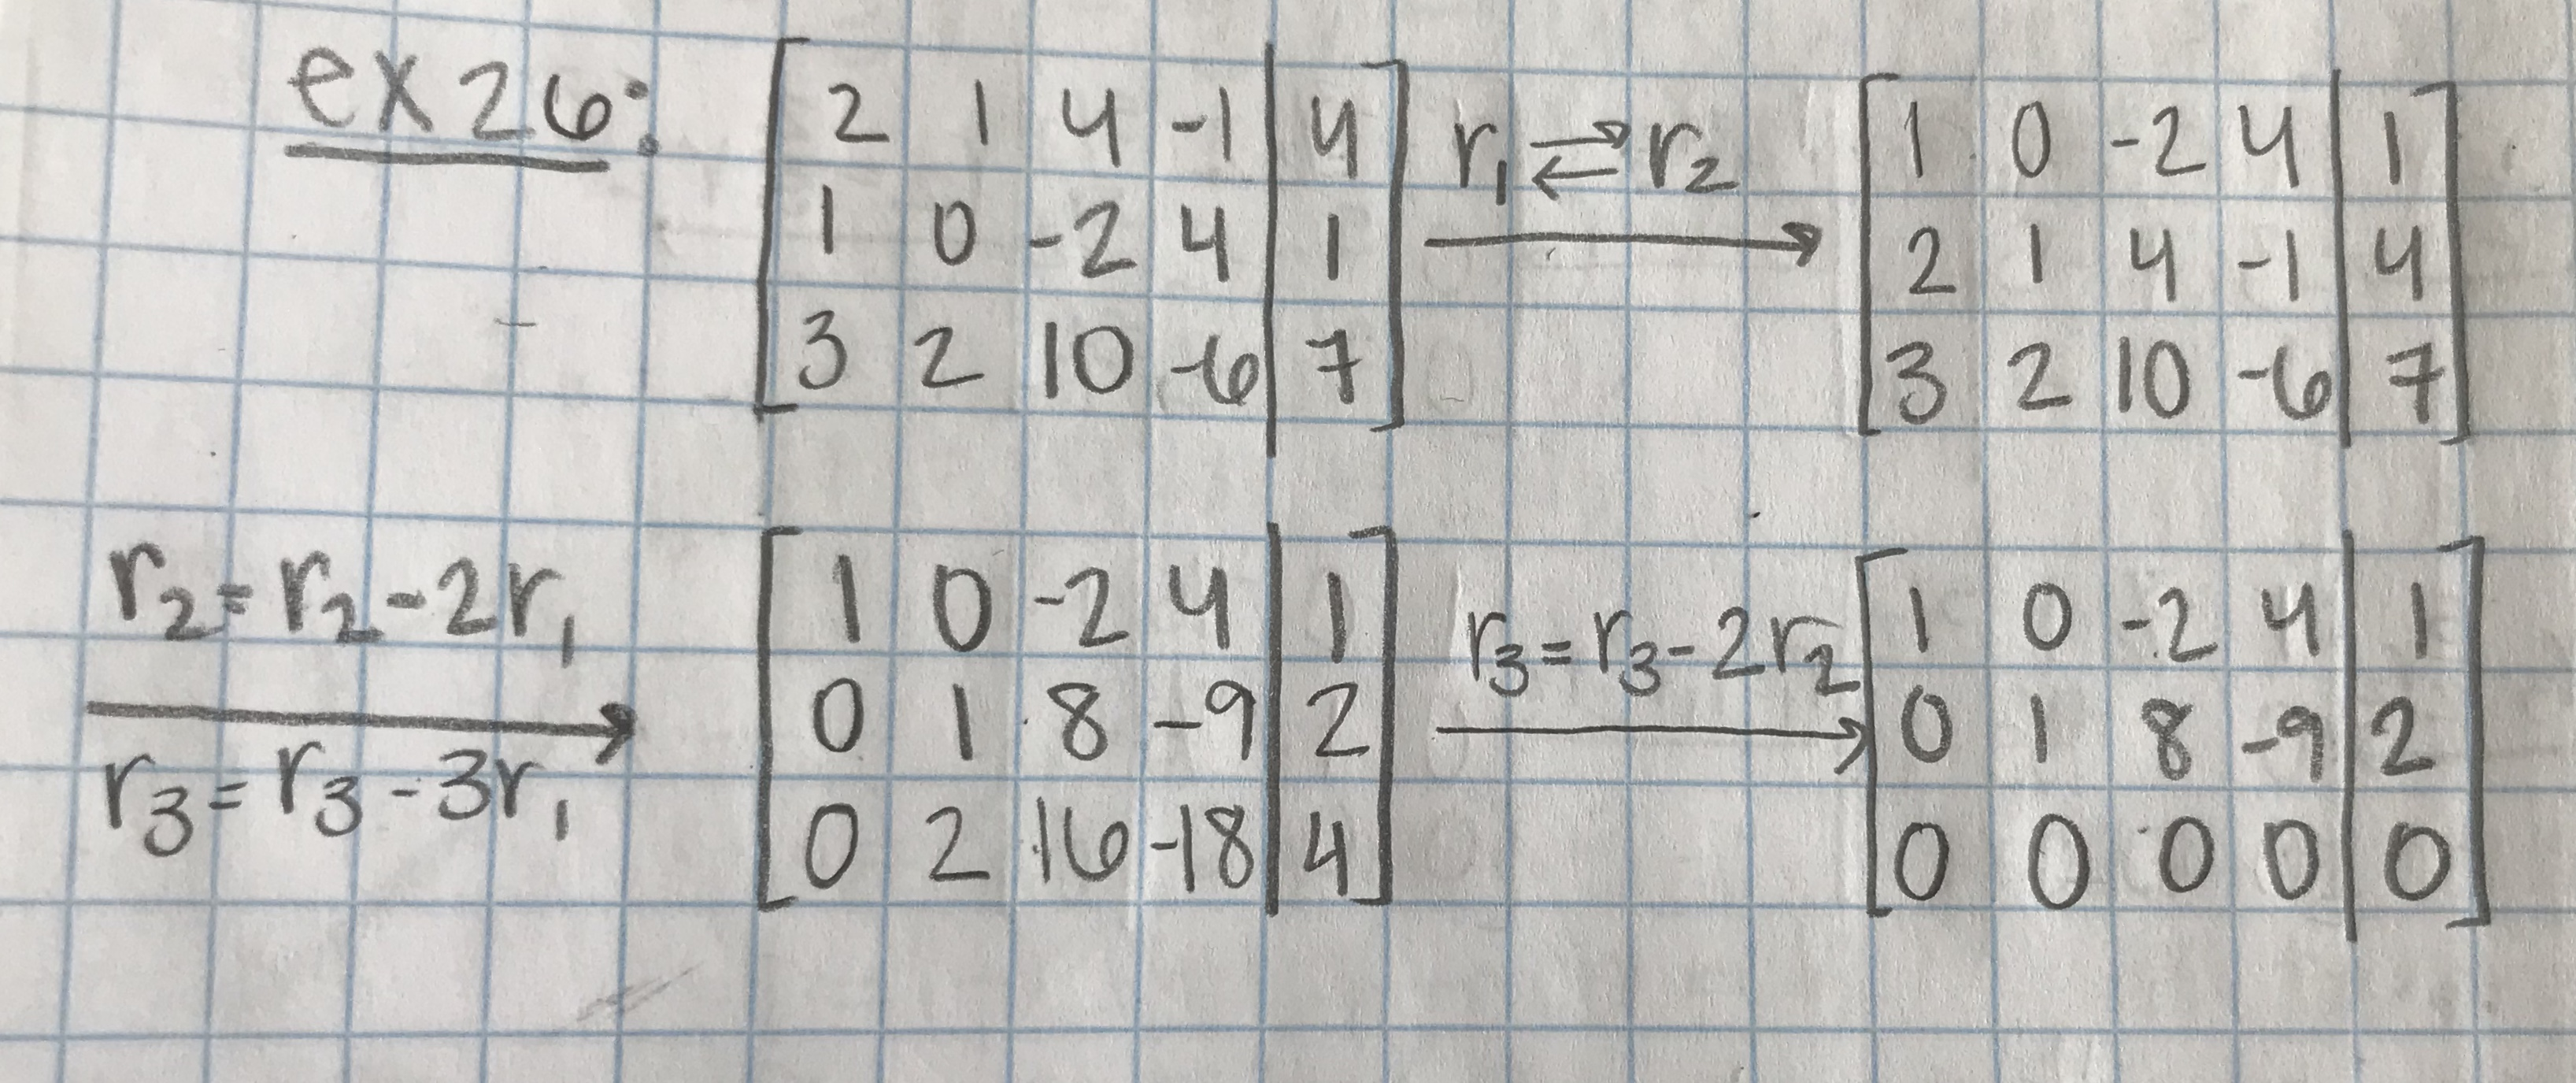
\includegraphics[scale=0.1]{exercise26}

\end{enumerate}

\end{document}